%!TEX root = ../dokumentation.tex

\chapter{Prototypische Implementierung}

\section{Bewegungserkennung}

Das Ziel der Bewegungserkennung ist es, nur sich bewegende Fahrzeuge zu analysieren und zu erkennen. Dieses Vorgehen wird mit Hilfe der OpenCV Hintergrundsubtraktion ermöglicht. 

Die Hintergrundsubtraktion (engl. \emph{background subtraction}) ist eine gängige und weit verbreitete Vorgehensweise zur Erzeugung einer Vordergrundmaske unter Verwendung statischer Kameras. Wie der Name besagt, berechnet die Hintergrundsubtraktion die Vordergrundmaske durch die Subtraktion zwischen dem aktuellen Bild und einem Hintergrundmodell, das den statischen Teil der Szene enthält, oder allgemeiner all das, was auf Grund der Eigenschaften der beobachteten Szene als Hintergrund betrachtet werden kann. 

\begin{figure}[htb]
	\centering
	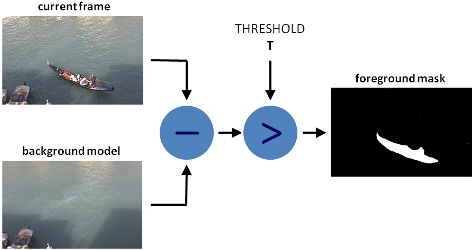
\includegraphics[width=\textwidth]{images/background_subtraction}
	\caption[Vorgehen der Hintergrundsubtraktion]{Vorgehen der Hintergrundsubtraktion \cite{opencv_bg_subtraction}}
\end{figure}

Im ersten Schritt wird ein anfängliches Modell des Hintergrundes berechnet, während im nächsten Schritt dieses Modell aktualisiert wird, um sich an mögliche Änderugungen in der Szene anzupassen. Der Schwellenwert (engl. \emph{threshold}) legt fest, was als Vordergrund anerkannt wird. Resultierend aus der Berechnung entsteht eine Vordergrundmaske. 

In diesem Prototypen wird eine Hintergrundsubtraktion mit dem \ac{MOG}2 Algorithmus durchgeführt. Dabei handelt es sich um einen Mixture-basierten Hintergrund-/Vordergrund Segmentierungsalgorithmus. \citeauthor{ZIVKOVIC2006773} führt diesen Algorithmus in den Arbeiten \citetitle{1333992} und \citetitle{ZIVKOVIC2006773} an \cites{1333992}{ZIVKOVIC2006773}. Eine wichtige Eigenschaft dieses Algorithmus ist die geeignete Anzahl von Gaußverteilungen für jeden Pixel. Er bietet somit eine bessere Anpassungsfähigkeit an wechselnde Szenen auf Grund von Beleuchtungsänderungen \cite{opencv_bg_subtraction2}. 

\vspace*{10mm}
\begin{lstlisting}[caption={Generation der Hintergrundsubtraktion}, label={lst:bgsub}]
# Generate background subtraction with opencv built-in methods    
fgbg = cv2.createBackgroundSubtractorMOG2(history=800, detectShadows=False, varThreshold=100)
\end{lstlisting}

Abbildung \ref{lst:bgsub} zeigt die Erstellung eines Hintergrundsubtraktionsobjekts für den Prototypen. Der Parameter \emph{history} wird dazu verwendet, um den Wert der Historie begrenzen zu können. Je höher dieser Wert ist, desto länger ist der Schweif den ein Objekt mit sich zieht. Für diesen Prototypen wurde die standardmäßige Schattenerkennung mit dem Parameter \emph{detectShadows} ausgeschaltet. Das Deaktivieren dieses Parameters führt zu einer deutlichen Leistungssteigerung des Algorithmus. \emph{varThreshold} ist ein Schwellenwert für den quadrierten Mahalanobis-Abstand zwischen dem Pixel und dem Modell. Dieser wird dazu verwendet, um zu entscheiden, ob ein Pixel durch das Hintergrundmodell gut beschrieben ist \cite{opencv_bg_subtraction3}. Bevor die Hintergrundsubktration auf das Video angewandt wird, muss das Video durch andere Hilfsfunktionen bearbeitet werden. Der erste Schritt zur genaueren Vorhersage ist die Grauskalierung \cite{cv_opencv}. 

Abbildung Grauskalierung

Eine Grauskalierung wird angewandt, da für die Bewegungserkennung keine Farbe benötigt wird und es zur Verbesserung der Anzeigequalität eines Bildes ohnehin zu einer Verminderung des Rauschens führt. 

\vspace*{10mm}
\begin{lstlisting}[caption={Graustufen auf das Video anwenden}, label={lst:grayscaling}]
# Apply grayscaling on video input
gray_frame = cv2.cvtColor(src=frame, code=cv2.COLOR_BGR2GRAY)
\end{lstlisting}

Mit Hilfe der in Abbildung \ref{lst:grayscaling} aufgeführten Funktion \emph{cvtColor} wird eine Grauskalierung des aktuellen Bildes durchgeführt. Der Parameter \emph{src} stellt das aktuelle Bild dar, auf welchem die Farbkonvertierung angewendet werden soll. \emph{code} übergibt eine OpenCV Konstante, die ein Color Space Conversion Code ist. Dieser Code gibt an, ob und was für eine Art der Farbtransformation durchgeführt werden soll. Die Konstante \emph{COLOR\_BGR2GRAY} stellt die Gewichtung der Veränderung von Farbkanälen dar (siehe Abbildung \ref{eq:rgbatogray} \cite{opencv_bg_subtraction4}). 

\begin{figure}[htb]
	\[\text{RGB[A] to Gray}: Y \leftarrow 0.299 * R + 0.587 * G + 0.114 * B \]
	\caption{Gewichtung der Farbkanäle}
	\label{eq:rgbatogray}
\end{figure}

Durch den in Abbildung \ref{eq:rgbatogray} aufgezeigten Vorgang wird die Multiplikation der einzelnen Farbkanäle dargestellt. Durch das multiplizieren der Kanäle mit der jeweiligen Konstante entsteht ein neuer RGB Wert $Y$. Dieser neue Wert kann im Anschluss auf das Bild angewandt werden, um eine Graustufierung zu ermöglichen \cite{opencv_bg_subtraction4}. Weitergehend wird auf das daraus entstandene Bild eine Gauß'sche Unschärfe eingesetzt. 

Da auch bei zwei unterschiedlichen, in sehr kurzem Abstand aufgenommenen Bildern, ein Unterschied der Beleuchtung oder dem Sensor der Kamera festgestellt werden kann, ist die Verwendung dieser Unschärfeapplikation von Nöten. 

\vspace*{10mm}
\begin{lstlisting}[caption={Anwendung des Weichzeichners}, label={lst:gaussianblur}]
# Application of Gaussian Blur
blur_frame = cv2.GaussianBlur(src=gray_frame, ksize=(3, 3), sigmaX=0)
\end{lstlisting}

Die Gauß'sche Unschärfe ist als ein $NxN$-Tap-Faltungsfilter definiert, der die Pixel innerhalb seines Footprints, basierend auf der Gauß-Funktion gewichtet. Die Unschärfefunktion ist definiert durch 

\begin{figure}[htb]
	\[G(x,y) = \frac{1}{2\pi \sigma^2}e^{-\frac{x^2+y^2}{2\sigma^2}}.\]
	\caption{Gauß'sche Unschärfefunktion}
	\label{eq:gaussian}
\end{figure}

Die Pixel des Filter-Footprints werden mit den Werten aus der Gauß-Funktion gewichtet und erzeugen so einen Unschärfe-Effekt. Die räumliche Darstellung des Gauß-Filters, zeitweise auch als \"{}Glockenfläche\"{} bezeichnet, zeigt, wie sehr die einzelnen Pixel des Footprints zur endgültigen Pixelfarbe beitragen \cite{rastergrid}.

\begin{figure}[htb]
	\centering
	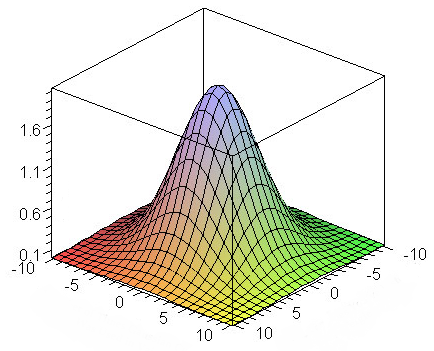
\includegraphics{images/gaussian_graph}
	\caption[Grafische Darstellung der zweidimensionalen Gauß-Funktion]{Grafische Darstellung der zweidimensionalen Gauß-Funktion\cite{rastergrid}}
	\label{fig:gaussian}
\end{figure}

Dieser Prototyp setzt einen 3x3 Kernel ein. Ein Kernel ist in diesem Anwendungsfall ein quadratisches Array von Pixeln. 
\begin{quote}
	\"{}Jedes Pixel im Bild wird mit dem Gaußschen Kern multipliziert. Dazu wird das mittlere Pixel des Kernels auf dem Bildpixel platziert und die Werte im Originalbild mit den Pixeln im Kernel multipliziert, die sich überlappen. Die aus diesen Multiplikationen resultierenden Werte werden addiert und dieses Ergebnis wird für den Wert am Zielpixel verwendet.\"{}\cite{qastack}. %TODO !! QUELLE FFS
\end{quote}

Je größer der Kernel ist, desto größer ist der Radius der Unschärfe und die Berechnungsdauer. Der $\sigma$-Wert der in Abbildung \ref{eq:gaussian} aufzeigten Gauß'schen Formel bestimmt die Standardabweichung der X- und Y-Richtung. Bei einem Wert von 0 wird die Standardabweichung anhand der Kernelgröße berechnet \cite{opencv_smoothing}. Nach der Minimierung des Rauschens kann anschließend die Hintergrundsubtraktion angewandt werden. 

\vspace*{10mm}
\begin{lstlisting}[caption={Anwendung der Hintergrundsubtraktion}, label={lst:bg_subtraction}]
# Application of background subtraction
fgmask = fgbg.apply(blur_frame)
\end{lstlisting}

Das Ergebnis der Hintergrundsubtraktion ist eine Vordergrundmaske, wie in Abbildung \ref{eq:gaussian} zu sehen. Die weiß markierten Stellen stellen den Vordergrund dar, wohingegen die schwarzen Stellen den Hintergrund hervorheben. 


\begin{figure}[htb]
	\centering
	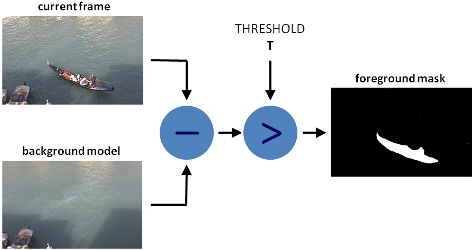
\includegraphics{images/background_subtraction}
	\caption{Erzeugung einer Vordergrundmaske}
	\label{fig:vordergrundmaske}
\end{figure}

Nachdem die beweglichen Elemente aus dem Video herauskristallisiert werden können, kann der Video Input für die Objekterkennung vorbereitet werden. Um dieses Ziel erfüllen zu können, wird die Vordergrundsubtraktion eingesetzt. 

\vspace*{10mm}
\begin{lstlisting}[caption={Dilation der Vordergrundmaske}, label={lst:foreground_dilation}]
# Application of foreground dilation
dilated_frame = cv2.dilate(src=fgmask, kernel=np.ones((3,3),np.uint8), iterations=3)
\end{lstlisting}

Eine Erweiterung, auch Dilation genannt, ist Bestandteil der mathematischen Morphologie. Die Morphologie ist eine Untergruppe der Bildverarbeitung. Dabei befasst man sich mit binären Bildern bzw. Rastergrafiken, also Bildern mit nur einem oder zwei Farbwerten \cite{Soille1998}. % TODO: Absolut sinnfreier Abschnitt
Durch die Dilation der Vordergrundmaske werden kleine schwarze Flecken zwischen weißen Flächen verdeckt, sowie die weißen Flächen größer und zu einer Region zusammengefasst. In Abbildung \ref{} sind bereits größere Strukturen von Objekten zu erkennen, dennoch sind ungewollte, kleinere Flächen sichtbar. Diese werden im nächsten Schritt gefiltert und entfernt. Um die kleineren weißen Flecken zu entfernen werden zunächst alle Konturen der digitalen Vordergrundmaske gesucht, wie in Abbildung \ref{} dargestellt. 

\vspace*{10mm}
\begin{lstlisting}[caption={Finden aller Konturen in der Vordergrundmaske}, label={lst:foreground_dilation_detection}]
# Contour detection of foreground mask
contours, _ = cv2.findContours(image=dilated_frame, mode=cv2.RETR_EXTERNAL, method=cv2.CHAIN_APPROX_SIMPLE)
\end{lstlisting}

Konturen können als eine Kurve erklärt werden, die alle kontinuierlichen Punkte entlang einer Begrenzung verbindet, die die gleiche Farbe oder Intensität besitzen \cite{opencv_contour}. Mit Hilfe der \emph{findContours} Funktion wird eine Liste aller gefundenen Konturen zurückgegeben. Die Kontur ist wiederum eine Liste von Koordinatenpunkten. Der Modus \emph{RETR\_EXTERNAL} gibt nur die extremen Außenkonturen, die eine Schmälerung der gefundenen Knoten mit sich bringt, zurück. Die Methode \emph{CHAIN\_APPROX\_SIMPLE} komprimiert horizontale, vertikale und diagonale Segmente und lässt deren Endpunkte zurück \cite{openstruct}. Um die Konturen auf das Video anzuwenden muss zunächst eine Maske des Videos erstellt werden (siehe Abbildung \ref{lst:mask_creation}).

\vspace*{10mm}
\begin{lstlisting}[caption={Erstellung einer Maske des aktuellen Bildes}, label={lst:mask_creation}]
# Create mask
mask = np.zeros_like(frame)
\end{lstlisting}

Unter Verwendung der \emph{zeroes\_like} Funktion des numpy Packages kann ein Array mit der Form und Größe des Bildes zurückgegeben werden. Dieses Array enthält nur Nullen und ist somit ein schwarzes Bild \cite{numpyzeroeslike}.
Die im Anschluss entstandenen Konturen können nun auf eine vorbestimmte Größe gefiltert werden. Hierfür wird die \emph{contourArea} Funktion verwendet (siehe Abbildung \ref{lst:contourmask}). Mit Hilfe eines Grenzwerts unter 1200 können kleinere, nicht relevante Konturen gefiltert und Objekte wie Personen oder Fahrräder auf der Straße erkannt werden. 

\vspace*{10mm}
\begin{lstlisting}[caption={Erstellen einer Konturenmaske}, label={lst:contourmask}]
# Draw rectangles around contours
for contour in contours:
            
    # Calculate the contour area. Skips small countours
    if cv2.contourArea(contour) < 1200:
        continue
                
    # Returns corners of contour. Doesn't consider the rotation of the object
    (x, y, w, h) = cv2.boundingRect(contour)
                        
    # draw filled contours in mask
    cv2.rectangle(img=mask, pt1=(x, y), pt2=(x+w, y+h), color=(255,255,255), thickness=-1)
\end{lstlisting}

Nach der Filterung der Konturen können die geraden Begrenzungsrechtecke mit Hilfe der \emph{boundingRect} Funktion ermittelt werden. Als gerades Begrenzungsrechteck ist ein Rechteck gemeint, das die Rotation eines Objekts außer Acht lässt. Diese Rechtecke werden als weiße Rechtecke auf die zuvor ermittelte Maske aufgetragen. Der Parameter \emph{thickness} füllt das Rechteck mit der angegebenen Farbe aus, sofern dieser den Wert -1 beinhaltet. 


Abschließend wird eine bitweise Verrechnung der Maske mit den im Video befindlichen Frames vorgenommen. Durch den $\cap$-Operator werden lediglich die weißen Stellen des Bildes hervorgehoben (siehe Abbildung \ref{} und \ref{}). Um diese Operation anwenden zu können müssen beide Bilder die selbe Größe und Form besitzen (siehe Abbildung \ref{lst:bitwise_operation}).

\vspace*{10mm}
\begin{lstlisting}[caption={UND-Operation der Maske und des aktuellen Bildes}, label={lst:bitwise_operation}]
# Bitwise and operation
movement_frame = cv2.bitwise_and(frame, mask)
\end{lstlisting}

Abbildung \ref{} zeigt das Ergebnis der Bewegungserkennung. Es werden nur Objekte, die sich im Video bewegen und groß genug für die Erkennung sind, angezeigt. Dies kann anschließend für die Objekterkennung verwendet werden. 

\section{Objekterkennung}

Um unterschiedliche Verkerhsteilnehmer wie Fahrräder, Autos und Motorräder wahrzunehmen, müssen diese Identifiziert und Erkannt werden. Unter Verwendung der Tensorflow Object Detection \ac{API} wird die Objekterkennung in diesem Prototyp umgesetzt \cite{tf_object_detection_github}. Die Tensorflow Object Detection API ist ein Open-Source Framework, welches auf Tensorflow aufbaut und das Konstruieren, Trainieren und Bereitstellen von Objekterkennungsmodellen erleichtert. Alle im Tensorflow Repository enthaltenen Modelle wurden anhand des \ac{COCO} 2017 Datensatzes trainiert. \ac{COCO} ist eine umfangreiche Objekterkennungs-, Segmentierungs- und Beschriftungsdatensatz Bibliothek mit über 330.000 Bildern und 91 Suchkategorien. Diese Modelle sind vor allem für Out-of-the-Box Inferenz nützlich, wenn die gewünschten Kategorien in den Datensätzen vorhanden sind. Objekte wie Fahrräder, Autos, Motorräder, LKWs und Busse sind bereits in den \ac{COCO} Datensätzen enthalten. Dies führt zu dem Anlass, ein bereits vortrainiertes Modell zu verwenden. Jedes Modell wird mit Hilfe der Geschwindigkeit in Millisekunden und der \ac{COCO} \ac{MAP} gemessen. Die Geschwindigkeit gibt an, wie lange ein Modell zur Erkennung von Objekten benötigt. Der \ac{COCO}-\ac{MAP} ist eine weitverbreitete Metrik zur Messung der Genauigkeit eines Modells. Je höher der \ac{MAP} Wert, desto genauer ist das Modell. Die Geschwindigkeit und der \ac{MAP} stehen häufig in Relation zueinander. % Quelle ?!
Auf Grund dieser Merkmale muss das zu wählende Modell mit den Anforderungen des Projektes zusammenpassen. Für die Echtzeiterkennung wird ein schnelles Modell mit geringer Genauigkeit benötigt. Für diesen Prototypen wurde sich für das Modell mit dem höchsten \ac{COCO}-\ac{MAP} Wert entschieden. Diese Wahl bringt eine durchaus hohe Einbuße der Erkennungsgeschwindigkeit mit sich, welche jedoch auf Grund der Verzichtbarkeit einer Echtzeiterkennung nicht weiter relevant ist. Neben Boxen (Umrandung des Objekts) können Modelle ebenfalls Keypoints zurückgeben, die für die weitere Kompatibilität mit Prototypen relevant ist. Bei der Keypoint Erkennung werden Personen erkannt und gleichzeitig deren Keypoint lokalisiert. Keypoints sind räumliche Orte bzw. Punkte im Bild, die definieren, was interessant ist oder im Bild hervorsticht. Sie sind invariant gegenüber Bilddrehung, -Schrumpfung, -Verschiebung und -Verzerrung \cite{kp_detection}.


% TODO: Fix footnote
\begin{figure}[htb]
	\centering
	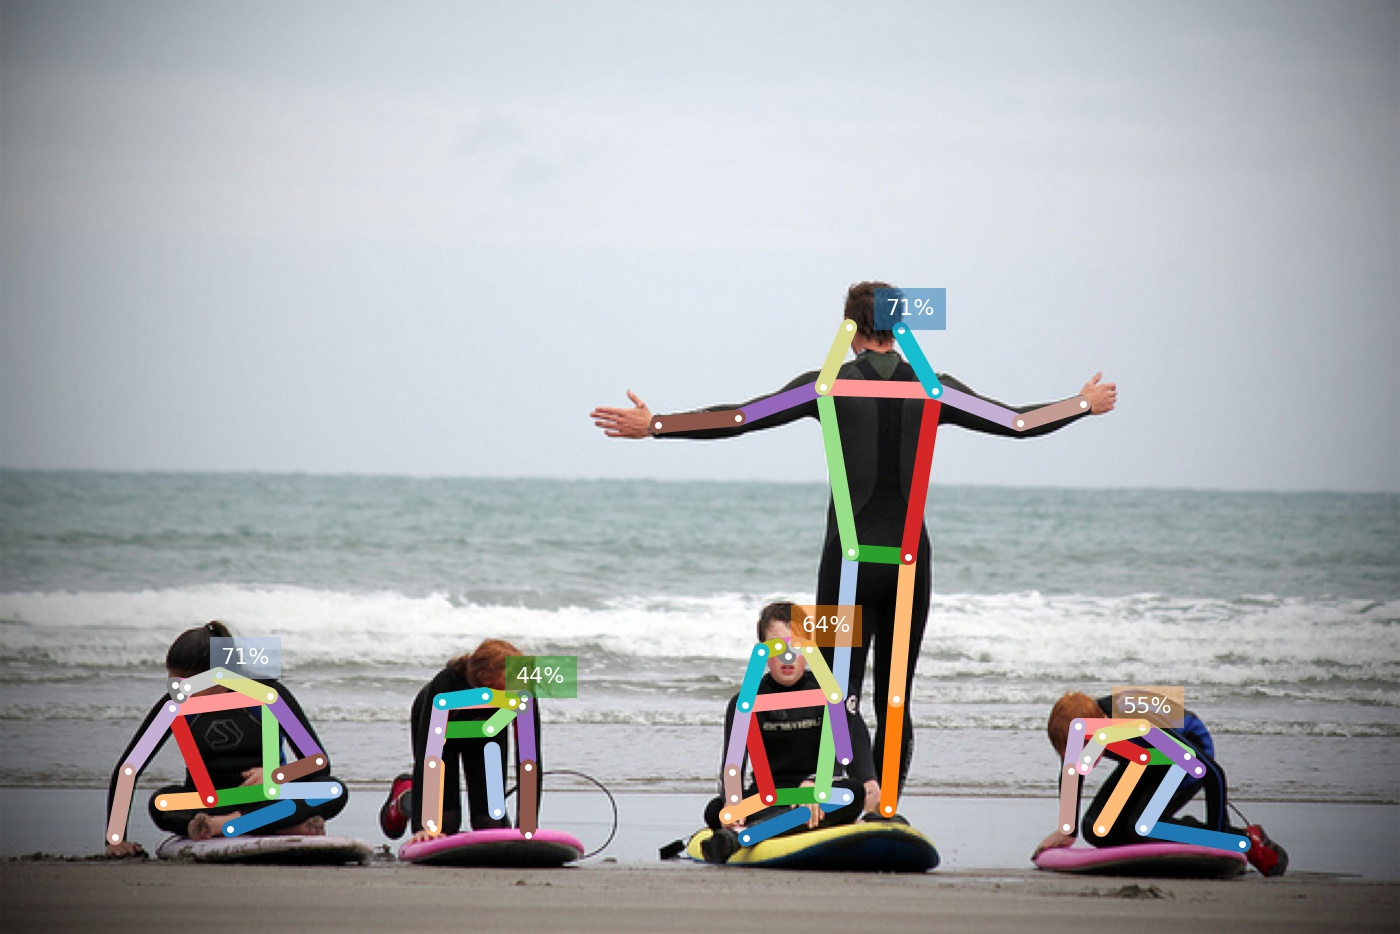
\includegraphics[width=.9\textwidth]{images/keypoint-detection}
	\caption[Keypoint Erkennung]{Keypoint Erkennung \footnote{https://raw.githubusercontent.com/openpifpaf/openpifpaf/main/docs/coco/000000081988.jpg.predictions.jpeg}}
	\label{fig:keypoint-detection}
\end{figure}

Für diesen Prototypen wird das EfficientDet-D7 Modell verwendet, das mit einem \ac{COCO}-\ac{MAP} Wert von 51,2 im Tensorflow Model Zoo ideal dazu geeignet ist, um die markantesten Objekte in einem Bild zu lokalisieren \cite{efficientdet}. EfficientDet ist die Objekterkennungs Variante des weitverbreiteten EfficientNet \cite{tan2019efficientnet} und baut auf dessen Erfolg auf. EfficientNets stammen aus einer Familie von Modellen, die eine hohe Leistung bei Benchmark-Aufgaben erreichen, während sie für eine Reihe von Effizienzparametern wie Modellgröße und \acp{FLOP} kontrolliert werden. Das Netzwerk wird in einer Reihe von Modellgrößen d0-d7 ausgeliefert. \acp{FLOP} bemisst die Anzahl an Gleitkommaoperationen pro Sekunde und ist ein Maß für die Leistungsfähigkeit eines Modells \cite{object_detection_comparison}. 

\begin{figure}[htb]
	\centering
	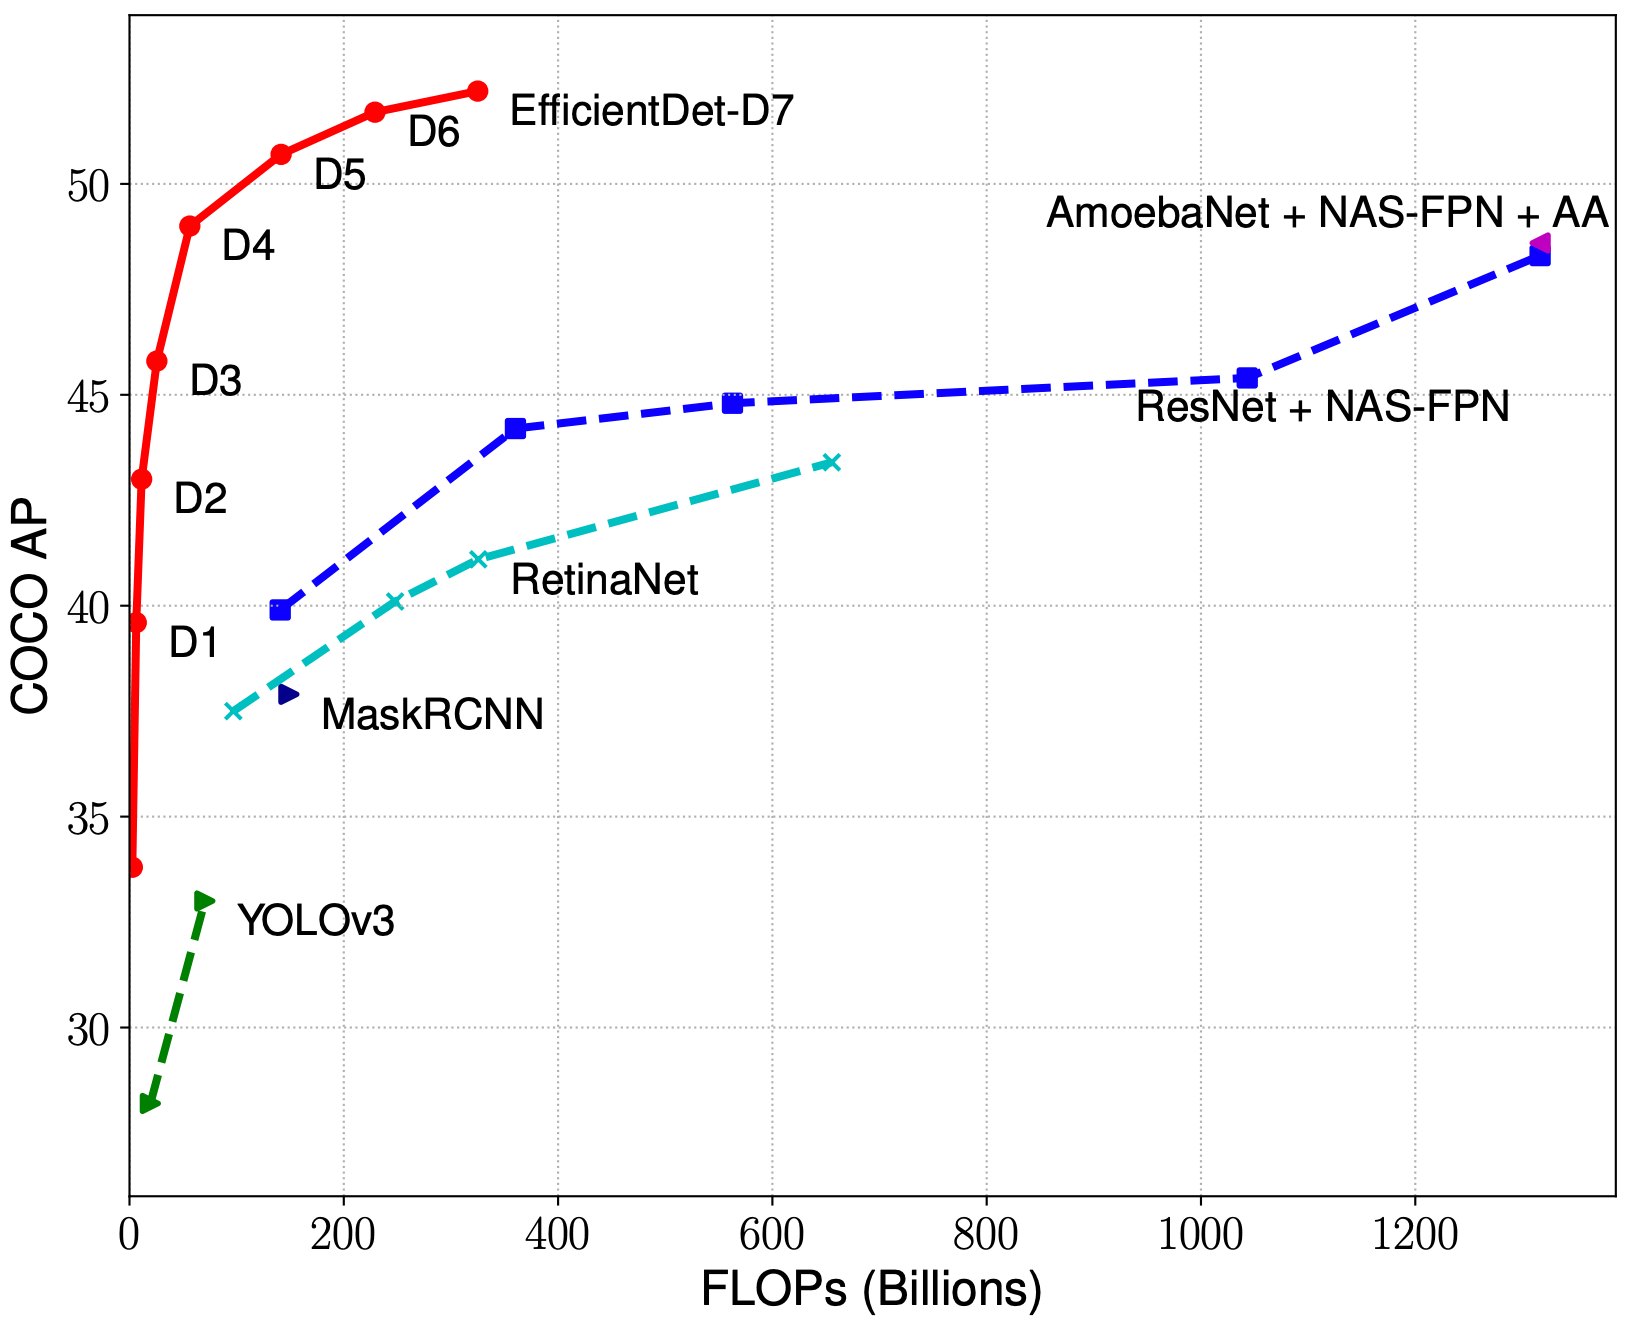
\includegraphics[width=\textwidth]{images/efficientdet}
	\caption[Modell FLOPs vs COCO Genauigkeit]{Modell \acp{FLOP} vs. \ac{COCO} Genauigkeit \cite{tan2020efficientdet}}
\end{figure}

EfficientDet erreicht die beste Leistung, mit der geringsten Anzahl von Trainingsepochen, unter den Objekterkennungsmodellen. Dies ist insbesondere von Vorteil, wenn mit begrenzter Rechenleistung gearbeitet wird \cite{solawetz}. Bevor das vortrainierte Modell verwendet werden kann, wird dieses als verpackte Datei heruntergeladen. Ebenfalls enthalten ist die zugehörige Beschreibungsdatei, welche eine Liste von Strings beinhaltet, die zur richtigen Beschriftung eines Objekts dient. Jede Beschriftung ist durch eine ID, die später zur Visualisierung verwendet wird, eindeutig erkennbar. Nach dem Herunterladen des Modells wird dieses extrahiert und mit der Beschreibungsdatei geladen \cite{obd_api}.
\vspace*{5mm}
\begin{lstlisting}[caption={Laden der Beschreibungsdatei mit anschließendem Erzeugen des Modells}, label={lst:loading}]
category_index = label_map_util.create_category_index_from_labelmap(use_display_name=True)
# Load pipeline config and build a detection model
configs = config_util.get_configs_from_pipeline_file(PATH_TO_CFG)
model_config = configs['model']
detection_model = model_builder.build(model_config=model_config, is_training=False)
\end{lstlisting}

Das Modell enthält zusätzlich eine Pipeline Konfigurationsdatei, welche zur Erzeugung des Modells verwendet wird. Eine Pipeline definiert Konfigurationen für ein Modell und automatisiert dadurch den Workflow des zu bauenden Modells. Pipelines für maschinelles Lernen bestehen aus mehreren aufeinanderfolgenden Schritten, die von der Datenextraktion und Vorverarbeitung bis hin zum Modelltraining und der Bereitstellung reichen \cite{valohai}.

\vspace*{10mm}
\begin{lstlisting}[caption={Laden der Checkpoints}, label={lst:checkpoints}]
# Restore checkpoint
ckpt = tf.compat.v2.train.Checkpoint(model=detection_model)
ckpt.restore(os.path.join(PATH_TO_CKPT, 'ckpt-0')).expect_partial()
\end{lstlisting}

Checkpoints erfassen den genauen Wert aller von einem Modell verwendeten Parameter \cite{tf_checkpoint}. Sodurch kann ein Modell wiederhergestellt und verwendet werden. Um nun eine Objekterkennung durchführen zu können, erwartet das EfficientDet-D7 Modell ein Dreikanalbild variabler Größe. Die Eingabewerte benötigen einen Tensor mit einer Höhe von 1 und einer Breite von 3 und zugehörigen Werten zwischen 0 und 255 \cite{efficientdet}. Auf Grund dieser Anforderung wird das Bild mit Hilfe der \gls{Numpy} Funktion \emph{expand\_dims} auf die erwartete Größe skaliert und in einen Tensor umgewandelt. Anschließend kann die Objekterkennung ausgeführt werden.

\vspace*{10mm}
\begin{lstlisting}[caption={Anpassung des Eingabetensors an das Modell}, label={lst:tensorfit}]
# Expand dimensions since the model expects images to have shape: [1, None, None, 3]
image_np_expanded = np.expand_dims(frame, axis=0)
input_tensor = tf.convert_to_tensor(image_np_expanded, dtype=tf.float32)
\end{lstlisting}

\begin{lstlisting}[caption={Ausführung der Objekterkennung}, label={lst:objectdetection_execution}]
# Execute object detection
detections, predictions_dict, shapes = detect_fn(input_tensor)
\end{lstlisting}

Die Funktion \emph{detect\_fn} gibt alle notwendigen Angaben als Python Dictionary zurück. Für den Prototypen werden die \emph{detection\_boxes}, \emph{detection\_scores} und \emph{detection\_classes} benötigt. \emph{Detection\_boxes} ist ein Tensor welcher die Koordinaten für 100 minimal umgebene Rechtecke, sogenannte Bounding Boxes, beinhaltet. Anhand dieser Koordinaten kann im späteren Verlauf der Objekterekennung die Umrandung der Objekte gezeichnet werden. 
 
\vspace*{10mm}
\begin{lstlisting}[caption={Beispielausschnitt der detection boxes}, label={lst:detectionbox_sample}]
'detection_boxes': <tf.Tensor: shape=(1, 100, 4), dtype=float32, numpy=
 array([[[0.4823483 , 0.33256257, 0.8408261 , 0.6648078 ],
         [0.39217225, 0.3756986 , 0.5196357 , 0.50812906],
         [0.482716  , 0.3359049 , 0.84076875, 0.6666065 ],
         [0.6159764 , 0.5550573 , 0.6771329 , 0.59031546],
         [0.39108938, 0.39384803, 0.43105263, 0.4248545 ]
\end{lstlisting}

Das zugehörige Objekt kann anhand des Indizes in der \emph{detection\_class} gefunden werden.

\vspace*{5mm}
\begin{lstlisting}[caption={Beispielausschnitt der detection classes}, label={lst:detectionclasses_sample}]
'detection_classes': <tf.Tensor: shape=(1, 100), dtype=int32, numpy=
 array([[ 2,  2,  7,  0,  0,  0,  2,  2,  7,  7,  2,  7,  2,  7,  2,  2,
          0, 26,  7,  5,  2,  7,  0,  2,  7,  0,  2, 30,  0,  0,  2,  2,
          0,  2,  5,  7,  2,  0, 36,  7,  7,  0,  2,  0,  9,  7, 13,  3,
         76,  7, 36, 61,  2,  2, 61,  7, 26, 61,  7,  2, 32, 13, 13,  0,
         17,  0, 32,  5,  5, 76, 27,  7,  7, 32, 26,  2,  7,  2,  9, 26,
         27,  0,  7, 13, 32, 33,  3,  2, 63, 43, 30, 13, 43,  1,  7, 13,
         30,  9,  2,  7]], dtype=int32)>,
\end{lstlisting}

Jede Zahl in dem \emph{detection\_classes} Tensor ist eine ID der in Auflistung \ref{lst:loading} geladenen Beschreibungsdatei. Ebenso kann anhand des Indizes die Genauigkeit der Erkennung in dem \emph{detection\_scores} Objekt abgefragt werden (siehe Auflistung \ref{lst:detectionscores_sample}).

\vspace*{5mm}
\begin{lstlisting}[caption={Beispielausschnitt der detection scores}, label={lst:detectionscores_sample}]
'detection_scores': <tf.Tensor: shape=(1, 100), dtype=float32, numpy=
 array([[0.65809727, 0.49682707, 0.32241914, 0.191383  , 0.16080539,
\end{lstlisting}

Das Dictionary \emph{detections} enthält weitere, nicht benötigte Ausgabe Parameter, die für diesen Prototypen jedoch irrelevant sind \cite{efficientdet}. Nicht alle Objekte die vom Modell erkannt werden, sind für die Objekterkennung notwendig. Daher werden die erkannten Objekte anhand der Klassen-ID gefiltert und aussortiert. Somit erhält man die Umrandungen, Klassen und Genauigkeiten eines einzelnen Bildes für die gewünschten Klassen. Die Visualisierung der Daten erfolgt in einem späteren Schritt. 

\section{Geschwindigkeitserkennung}

\section{Fahrtrichtungserkennung}






